\subsection{Use Case Diagram}
	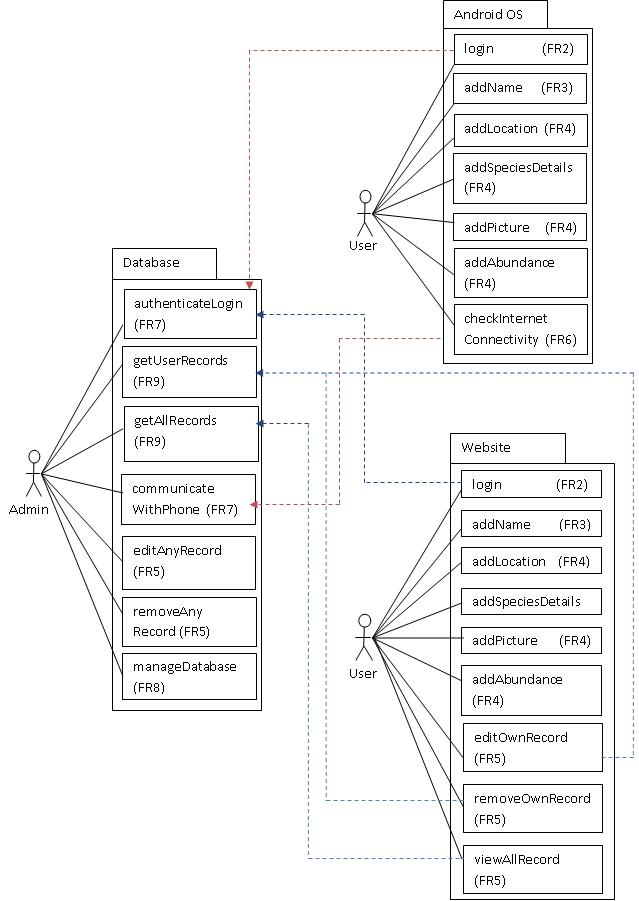
\includegraphics[scale=0.8]{useCases/useCase.png}
\subsection{Use Case Descriptions}

	\subsubsection{Android OS User}
	\begin{tabular}{| l  r | p{10cm} |}
		\hline
		FR2 & login  & User should be able to log into the application by entering a valid username\\ \hline
		FR3 & addName  & User should be able to add the name of a plant to the database \\ \hline
		FR4 & addLocation  & User should be able to add the location of a plant to the database \\ \hline
		FR4 & addSpeciesDetails  & User should be able to add a description of the plant to the database \\ \hline
		FR4 & addPicture  & User should be able to add a picture of the plant to the database \\ \hline
		FR4 & addAbundance & User should be able to record the level of abundance of the plant within the area \\ \hline
		FR6 & checkInternetConnectivity  & The application should be able to know if it is connected to the internet and is able to send records to the database. If not the data is stored in local storage \\ \hline
	\end{tabular} \\

	\subsubsection{Website user}
	\begin{tabular}{| l  r | p{10cm} |}
		\hline
		FR2 & login  & User should be able to log into the application by entering a valid username\\ \hline
		FR3 & addName & User should be able to add the name of a plant to the database \\ \hline
		FR4 & addLocation  & User should be able to add the location of a plant to the database \\ \hline
		FR4 & addSpeciesDetails  & User should be able to add a description of the plant to the database \\ \hline
		FR4 & addPicture  & User should be able to add a picture of the plant to the database \\ \hline
		FR4 & addAbundance & User should be able to record the level of abundance of the plant within the area \\ \hline
		FR5 & editOwnRecord  & User should be able to make changes to any record that they have added to the database \\ \hline
		FR5 & removeOwnRecord  & User should be able to remove any record that they have added to the database \\ \hline
		FR5 & viewAllRecord  & User should be able to view any record in the database through the website \\ \hline
	\end{tabular} \\

	\subsubsection{Admin}
	\begin{tabular}{| l  r | p{10cm} |}
		\hline
		FR7 & authenticateLogin  & The server will allow a user to log onto the application through their phone or through the website providing that the user has entered correct username and/or password. Using a database which contains details of valid usernames and passwords \\ \hline
		FR9 & getUserRecords  & When the user wants to view edit or delete records they have entered the server will need to call them from the database \\ \hline
		FR9 & getAllRecords  & The server will send information about all the records in the database to the user upon request \\ \hline
		FR9 & communicateWithPhone  & Server must be able to send and receive data from the phone of records being entered \\ \hline
		FR5 & editAnyRecord  & The website admin should be able to edit any record entered in the database by any user \\ \hline
		FR5 & removeAnyRecord  & The website admin should be able to remove any record entered into the database by any user \\ \hline
		FR8 & manageDatabase  & The database administrator will be able to log into the database and manage/maintain it \\ \hline
	\end{tabular}
